\newpage
\section*{Exercise 2 }

\subsection*{Histograms and implementations (Qahir)}
The histogram for 10000 samples of the different distributions along with the true pdf can be seen on figure \ref{fig:ex21}. It can be seen that all of the methods except for the Alias for the 6 point distribution sample well from the true distribution. The reason for this is that the Alias table does not correspond well to the actual distribution. As an example consider $X=5$ for which $p=1/4$ and this is the 2nd highest probability for the observations. But in the alias tables we have $F(5)=1/4$ (the lowest value) and none of the $L(\cdot)$ points towards $5$. Hence there is not a good correspondence. For the code see the appendix. 


\begin{figure}[H]
        \centering
        \begin{subfigure}[H]{0.475\textwidth}
            \centering
            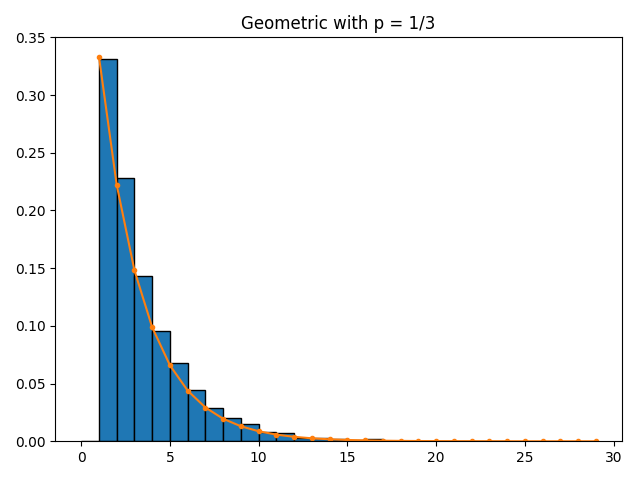
\includegraphics[width=\textwidth]{geo.png}
            \caption[Network2]%
            {{\small Geometric with $p=1/3$}}    
            \label{fig:mean and std of net14}
        \end{subfigure}
        \hfill
        \begin{subfigure}[H]{0.475\textwidth}  
            \centering 
            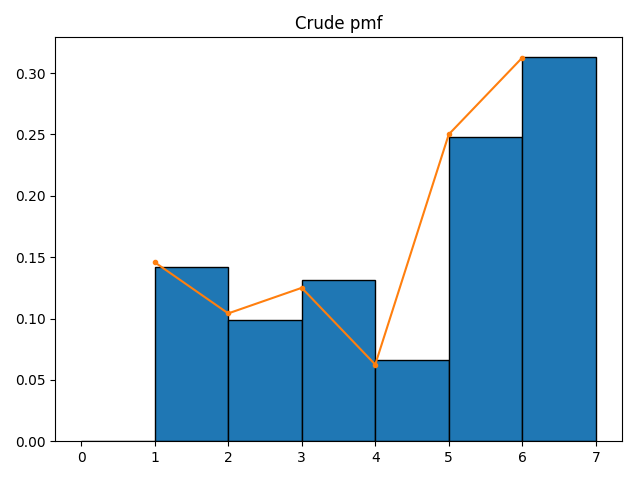
\includegraphics[width=\textwidth]{crude.png}
            \caption[]%
            {{\small Crude for 6-point}}    
            \label{fig:mean and std of net24}
        \end{subfigure}
        \vskip\baselineskip
        \begin{subfigure}[H]{0.475\textwidth}   
            \centering 
            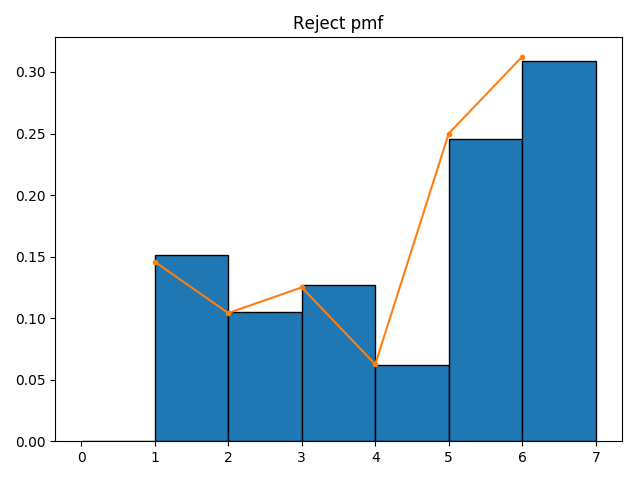
\includegraphics[width=\textwidth]{reject.png}
            \caption[]%
            {{\small Rejection for 6-point}}    
            \label{fig:mean and std of net34}
        \end{subfigure}
        \quad
        \begin{subfigure}[H]{0.475\textwidth}   
            \centering 
            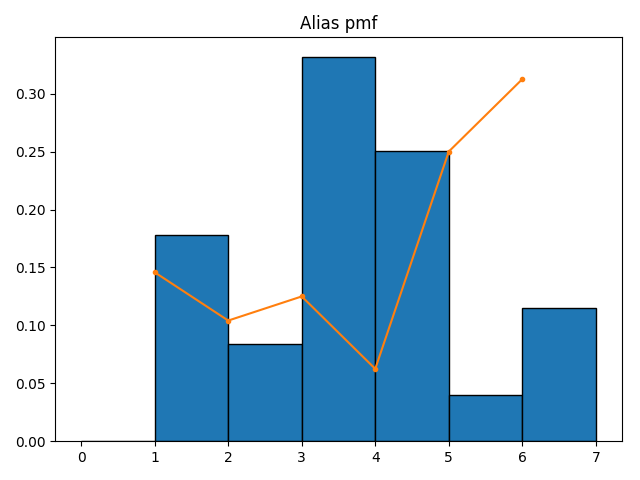
\includegraphics[width=\textwidth]{alias.png}
            \caption[]%
            {{\small Alias for 6-point}}    
            \label{fig:stuff}
        \end{subfigure}
        \caption[ The average and standard deviation of critical parameters ]
        {\small Histogram of different sampling methods (blue) - the orange dots indicate the true probability mass function} 
        \label{fig:ex21}
    \end{figure}





\subsection*{$\chi^2$ test(Sen)}
The $\chi^2$ test results are shown in table \ref{tab:discreteTest}. For the alias method, the p value is lower than 0.05, therefore we reject the null hypothesis.
\begin{table}[h]
    \centering
    \begin{tabular}{|c|c|c|c|}
    \hline 
    case & degree of freedom & T statistic & p \\ \hline
      Geometric distribution  &  23 & 19.55 & 0.6689\\  \hline
      Crude 6-point   & 5 &4.11& 0.5337\\ \hline
      Reject 6-point &5 & 1.70 & 0.8889\\ \hline
      Alias 6-point & 5 & 12268 & 0\\ \hline
    \end{tabular}
    \caption{$\chi^2$ test for discrete variable simulation}
    \label{tab:discreteTest}
\end{table}